
\chapter{Hidden variables for semiclassical models with state-dependent forces}

Hidden variable theories [CITE, CITE] are interpretations of quantum mechanics which posit that there are definite states underlying quantum wavefunctions, such that quantum indeterminacy is an illusion---an emergent phenomenon rather than a fundamental fact. The Bell inequality [CITE] proves that any such theory must be \emph{nonlocal} in order to explain all the predictions of quantum mechanics, and perhaps in light of this, most physicists surveyed [CITE] do not believe that hidden variables underlie physical reality.

However, by framing quantum systems in classical terms, hidden variable theories can provide an excellent computational tool for \emph{approximate} models of quantum systems, when it is reasonable to approximate some degrees of freedom as classical, yet other degrees of freedom need to be modelled quantum mechanically. Just as hidden variable theories have framed the quantum world in terms that are agreeable to the classical view of the world in the minds of some interpreters of quantum mechanics, so can they bridge the gap between a \emph{simulated} quantum world and a \emph{simulated} classical world coexisting in the same computer simulation.

In this chapter I describe what I call the `hidden variables semiclassical' (\textsc{hvsc}) method: a method of combining quantum simulations with classical simulations, with hidden variables bridging the gap between the classical and quantum degrees of freedom. In this introduction I describe existing semiclassical methods, the manner in which their quantum and classical parts are typically coupled based on expectation values (which I'm calling the `Ehrenfest method'), and in which regimes this inaccurate---namely the Stern--Gerlach experiment and similar situations in which considerable entanglement between motional and internal degrees of freedom develop.

In [SECREF THE NEXT SECTION] I give the technical definition of a hidden variable theory, and motivate the use of such a theory for coupling quantum and classical degrees of freedom in such a way that the a semiclassical model can be made to agree more closely than the Ehrenfest method with the underlying fully quantum model it is approximating, and ultimately, with experiment.

In section [SECREF THE SECTION AFTER THAT] I then go into the implications of welcoming a hidden variable into a semiclassical model, including additional required assumptions and approximations, and I derive the equations of motion for the model as a whole. Then in section [SECREF] I discuss the method further including its limitations.

Throughout this chapter, I make comparison between the \textsc{hvsc} and Ehrenfest methods. The two methods share most of the same flaws, save for \textsc{hvsc}'s ability to reproduce the Stern--Gerlach experiment. As such \textsc{hvsc} is an incremental improvement on the Ehrenfest method that solves this one specific problem. My method has a number of crude approximations---namely that wavepackets have a fixed size and that the decoherence of the atom's internal state is Markovian---and the wavepacket size and decoherence rate are estimated using approximate formulae. While crude, this is nonetheless an improvement over the Ehrenfest method's implicit assumption that decoherence does not occur at all (in which case the wavepacket size does not matter, as I will show), which is considerably less correct than even the crudest calculation of a Markovian decoherence rate. The \textsc{hvsc} method forces these assumptions to be made explicit, and serves as a minimal improvement to the Ehrenfest method, taking into account the simplest kind of decoherence only. Further improvements to the method are likely possible, but would be computationally more intensive to implement and unlikely to be worth it given the typical accuracy demanded of semiclassical simulations.


\subsection{Semiclassical models}

A semiclassical model is any model in which some degrees of freedom are treated quantum mechanically, and others classically. The most common combination is that of treating an atom's internal electronic state quantum mechanically and its motional degree of freedom classically. This is useful whenever the quantum effects of the atom's motion are not of interest, for example if temperatures are high and thus atomic wavelengths are short---such that quantum effects simply aren't visible in the motion of the particles and so they can accurately be modelled as classical billiard balls. The energy gaps between different electronic states are so large however that only at very high temperatures (at which atoms ionise anyway) do they start to appear as a continuum compared to thermal energy scales, and the interaction of different spin states of the atom with different optical and magnetic fields does not make them appear as classical continua either. Thus, quantum effects can be ignored for centre of mass motion of the atom, but not for the relative motion of its electrons with respect to the nucleus, or for the nuclear and electronic spin degrees of freedom.

In this regime, atoms are often modelled semiclassically, with these internal degrees of freedom modelled using a state vector $\ket\chi$ evolving according to a Hamiltonian $\hat H$ via the Schr\"odinger equation, and the centre of mass motion modelled as a position $\vec r$ and velocity $\vec v$ evolving according to Newton's second law (\figref{fig:semiclassical}).

\begin{figure}[t]
    \centerfloat
    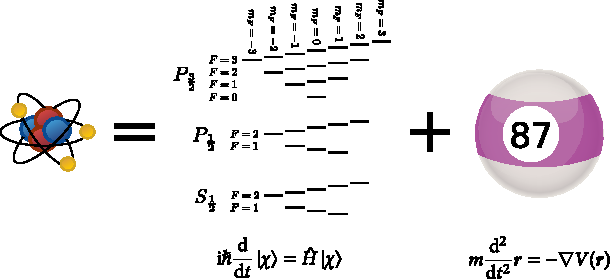
\includegraphics[width=0.75\textwidth]{figures/hidden_variables/semiclassical.pdf}
    \caption{Artist's depiction of a semiclassical atom.}
    \label{fig:semiclassical}
\end{figure}

Once one has defined a potential function $V(\vec r)$ and a Hamiltonian (also possibly varying with space) $\hat H(\vec r)$, and other possible additions\footnote{Such using a Monte-Carlo wavefunction method [CITE, SECREF?] to model the effect of spontaneous emission on $\ket\chi$, and modifying $\vec v$ instantaneously by a random-direction recoil velocity upon each photon emission}, ones job is done and the rest can be left to numerical differential equation solvers to evolve some concrete vector representation $\vec\chi$ of $\ket\chi$ as well as the state variables $\vec r$ and $\vec v$ for motional degree of freedom in time according to the coupled differential equations
\begin{align}\label{eq:simple_semiclassical_first}
\dv{t}\ket\chi &= -\frac\ii\hbar \hat H(\vec r)\ket\chi,\\
\dv{t}\vec v &= -\frac1m\nabla V(\vec r),\\
\dv{t}\vec r &= \vec v\label{eq:simple_semiclassical_last}.
\end{align}
In the next subsection I explain why it's not always that simple.

\subsection{Stern--Gerlach separation and evaporative cooling}

In the Stern--Gerlach experiment [CITE], particles with quantum spin and a magnetic moment---atoms for example---are fired as a beam through a region of space with a magnetic field gradient. The well known result is that two clusters of positions (if the atoms are spin $\frac12$) are observed once the beam emerges, rather than a continuous smear of positions, indicating that angular momentum---like many quantities in quantum mechanics---is quantised.

This is the case even if one spin-polarises the particles before they are passed through the magnetic field gradient, say putting them in an eigenstate of the $\hat F_x$ operator. Then, if the magnetic field is along the $z$ direction, and the gradient is also in the $z$ direction, two clusters of positions are also observed, even though all particles were in the same state when they entered the region in which there was a magnetic field gradient. This is a display of the indeterminacy of quantum mechanics: even though all particles had the same initial state, there were nonetheless different outcomes for each particle.

The Stern--Gerlach effect is a consequence of quantum mechanics, to be sure, but it has little to do with the wave nature of the atoms. If we introduced some double slits for the atoms to pass through in addition to the magnetic field gradient, then we would be seeing the wave nature of the atoms as interference patterns at the detection screen at the end of the experiment. But if we do not, and if the particles have short de-Broglie wavelengths, then quantum mechanics is not apparent in the motion of the particles through space---except via the influence of spin on seemingly choosing one trajectory or the other. The effect is well understood quantum mechanically, but is difficult to model semiclassically because even if we are happy to approximate wavepackets as small, the wavepackets do not take a single trajectory. Rather they split into two wavepackets, with the part of the superposition corresponding to one spin projection state (along the direction of the local magnetic field) moving one way, and the part of the superposition with the other spin projection going the other way. The trajectories can still be sill quite classical, it's just that there are two of them.

A similar situation exists in \textsc{rf} evaporative cooling (Section \ref{sec:evaporative_cooling}) of cold atoms en-route to \textsc{bec}. Atoms are trapped in a magnetic trap, and are spin polarised so as to be fully spin down (for $^{87}$Rb this is the trapped state) with respect to the local magnetic field at the position of each atom. The magnetic field's direction---not just  its magnitude---varies in space, and so different atoms have different spins, but they are all spin down with respect to the quantisation axis of the local magnetic field.\footnote{Out of habit we are already speaking semiclassically---to talk about the atoms' position is to assume they have one---and yet we're describing their spin quantum mechanically}. As the atoms move through space, they move in orbits---punctuated by collisions---about the magnetic field zero at the centre of the trap, since they feel a force $F\propto-\nabla\abs{\vec B}$ due to the gradient of the Zeeman potential. Provided they are moving slowly (specifically, provided their Larmor precession period is short compared to the time the magnetic field as seen by the atom takes to change by a non-negligible fraction of its current value), the atoms' spins adiabatically follow the local field and remain spin-down, even as the field as seen by each atom fully reverses its direction every half orbital period.

Near the centre of the trap where the atoms are moving faster, the fields are small and therefore have large fractional derivatives and lead to large Larmor periods, adiabaticity no longer holds and the atoms may make spin transitions with respect to their local magnetic field. Once an atom passing close to the fiels zero has evolve into a superposition of spin projection states with respect to the local field, it is in a situation identical to the initial condition of the Stern--Gerlach experiment, causing the spin projection components to spatially separate in the magnetic field gradient. The spin up component is anti-trapped and repelled from the centre of the trap, and the zero spin projection component (since the groundstate of $^{87}$Rb is spin-$1$) feels no force and moves in a straight line. The spin down component continues on an orbit about the field zero which is just as tight as before, unaffected by the close approach to the field zero other than being reduced in amplitude. Eventually a collision occurs, either with other atoms or with the walls of the vacuum system and the wavefunction collapses to choose one of these options, leading to atoms probabilistically leaving the trap (called Majorana losses [CITE]) or remaining trapped. Again, the trajectories can still be quite classical, it's just that there are three of them, and which is taken is probabilistic.

How can we model these effects semiclassically? Equations \eqref{eq:simple_semiclassical_first} to \eqref{eq:simple_semiclassical_last} are not sufficient, because exists no single classical potential $V(\vec r)$ that can describe the motion of the atoms. Rather, the atoms feel a different force depending on which spin state they are in. Just as the Hamiltonian can be a function of space, so can the potential be a function of the internal state of the atom: $V = V(\vec{r}, \ket\chi)$. Ehrenfest's theorem states that [CITE]
\begin{align}
m\dv[2]{t}\ev{\hat{\vec r}} = - \ev{\nabla \hat V},
\end{align}
where the expectation values are over all degrees of freedom, not just motional. If we approximate a small wavepacket centred at the position $\vec r$ in order ignore the wave nature of the atoms, this becomes:
\begin{align}
m\dv[2]{t} \vec r = - \nabla \matrixel{\chi}{\hat V(\vec r)}{\chi},
\end{align}
where the operator $\hat V(\vec r)$ now only acts on the subspace of the internal state of the atom, since we have already taken an expectation value over (a small region of) space. Provided all potentials the atom is subjected to are included in the Hamiltonian for its internal state (including any energy offsets that do not
depend explicitly on the internal state), this is nothing but
\begin{align}
m\dv[2]{t} \vec r = - \nabla \matrixel{\chi}{\hat H(\vec r)}{\chi},
\end{align}
where $\hat H$ is the Hamiltonian describing the evolution of the atom's internal state. We now can construct the \emph{Enhrenfest semiclassical method} describing how the \emph{expectation value} of a well localised atom's position evolves with time:

\begin{align}\label{eq:ehrenfest_semiclassical_first}
\dv{t}\ket\chi &= -\frac\ii\hbar \hat H(\vec r)\ket\chi,\\
\dv{t}\vec v &= -\frac1m\matrixel{\chi}{\hat H(\vec r)}{\chi},\\
\dv{t}\vec r &= \vec v\label{eq:ehrenfest_semiclassical_last}.
\end{align}

The Ehrenfest semiclassical method is the same as the simple semiclassical method~\eqref{eq:simple_semiclassical_first} to~\eqref{eq:simple_semiclassical_last}, except that it has an answer to the question ``What should we use for $V(\vec r)$ when the atom is in a superposition of states that feel different potentials?'', which is ``use the expectation value''. 

This is all well and good if the expectation value of position is a good approximation to the situation being modelled. But in the Stern--Gerlach experiment and Majorana losses in magnetic traps, the expectation value of position is a poor match to reality. In the Stern--Gerlach experiment beginning with spin-polarised atoms, this would result in a single blob in the middle of the screen, rather than two. And in an atom approaching the field zero in a magnetic trap, it would result in the atom broadening its orbit somewhat, rather than splitting into multiple possible trajectories (Figure \ref{fig:evap_problem}). Semiclassical simulations of evaporative cooling performed by Christopher Watkins [CITE] displayed an unphysical heating of the atom cloud that I believe is due to the Ehrenfest method's inability to model Stern--Gerlach separation. In a real magnetic trap during evaporative cooling to Bose--Einstein condensation, the mean free path is large enough that the part of the wavepackets that are no longer trapped will usually leave the trap without colliding with any other atoms. This means that the energy the untrapped and anti-trapped components have gained relative to the trapped component moving away from the field zero is not usually shared with other atoms upon collision---the extra energy leaves with the atoms. However, if a close approach to the magnetic field zero merely means a broadening of the atoms orbit, then the extra energy does not leave as fast, if at all, and can be shared with other atoms via collisions, turning what would have been an atom loss effect into an overall gradual heating of the cloud. 

\begin{figure}[t]
    \centerfloat
    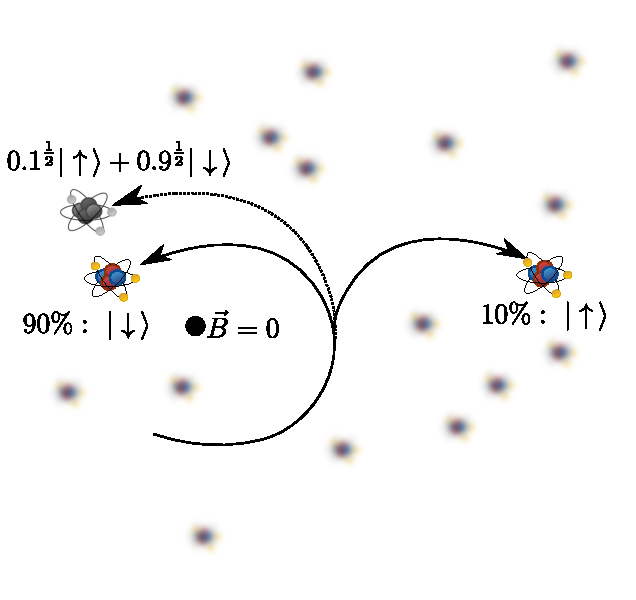
\includegraphics[width=0.75\textwidth]{figures/hidden_variables/evap_problem.pdf}
    \caption{todo}
    \label{fig:evap_problem}
\end{figure}

So how can we modify a semiclassical method to choose only one trajectory? Firstly, since each trajectory corresponds to one of the internal states (though some might be degenerate), our model must choose an internal state and use the classical trajectory corresponding to that internal state only. Secondly, since all atoms begin in identical states and yet some take one trajectory and some another, this choice must be probabilistic. Finally, the probabilities must be consistent with those from quantum mechanics, i.e. the Born rule: the probability of an atom taking each trajectory must be proportional to the squared amplitude of the internal state of the atom, projected onto the eigenstate corresponding to that trajectory.

There exists a category of theories dealing with precisely this question of how to choose a specific state of a quantum system in a stochastic way, such that the probability of having chosen a state is equal to that given by quantum mechanics. Such theories are called ``hidden variable'' theories, and the number specifying which state has been chosen is the ``hidden variable''.

\section{Hidden variable theories}

In his paper \emph{Quantum computing and dynamical quantum mdels}, Aaronson defines a ``dynamical quantum model''[CITE]:

\begin{quote}
A \emph{dynamical quantum model} assigns an eigenstate to a specified observable even when no measurement is made, and gives a stochastic evolution rule for that eigenstate. Such a model yields a distribution of classical histories of a quantum state
\end{quote}
In a later paper, \emph{Quantum computing and hidden variables}, superseding the first, Aaronson renames dynamical quantum models \emph{hidden-variable theories} and instead defines:
\begin{quote}
For us, a hidden-variable theory is simply a way to convert a unitary matrix that maps one quantum state to another, into a stochastic matrix that maps the initial probability distribution to the final one in some fixed basis
\end{quote}
This is what a hidden-variable theory is for the purposes of this chapter as well. Though the second paper supersedes the first, the definition it gives is more tangible for us---we wish to \emph{assign an eigenstate} to our atoms (choose one of the internal states in order to decide which trajectory to follow), and have a \emph{stochastic evolution rule} for which eigenstate is chosen at any one time (allow the atom to begin taking a different trajectory if it makes transitions between states).

But the second definition is more specific. The stochastic evolution rule is in the form of a stochastic matrix, with elements equal to transition probabilities for some time interval. And the rule should be in some way based on the unitary evolution that the quantum system evolves according to in the same interval of time, such that the initial and final probabilities of the stochastic matrix and unitary evolution agree. That is, if a quantum state $\ket\chi$ evolves in a certain basis $\{\ket{n}\}$according to a unitary $\hat U(t^\prime, t)$:
\begin{align}
\left[\begin{matrix}
\chi_1(t^\prime)\\\chi_2(t^\prime)\\\chi_3(t^\prime)\\\vdots
\end{matrix}\right]
= \left[\begin{matrix}
U_{11}(t^\prime, t) & U_{12}(t^\prime, t) & U_{13}(t^\prime, t)&\hdots\\
U_{21}(t^\prime, t) & U_{22}(t^\prime, t) & U_{23}(t^\prime, t)&\hdots\\
U_{31}(t^\prime, t) & U_{32}(t^\prime, t) & U_{33}(t^\prime, t)&\hdots\\
\vdots & \vdots & \vdots & \ddots
\end{matrix}\right]
\left[\begin{matrix}
\chi_1(t)\\\chi_2(t)\\\chi_3(t)\\\vdots
\end{matrix}\right],
\end{align}
where $\chi_n = \braket{n}{\chi}$ and $U_{nm}(t^\prime, t) = \matrixel{n}{\hat U(t^\prime, t)}{m}$, then a hidden variable theory is a matrix-valued function $S(U(t^\prime, t), \vec\chi(t)))$, where $\vec\chi(t)$ and $U(t^\prime, t)$ are the vector and matrix representations of the state vector $\ket\chi(t)$ and unitary $\hat U(t^\prime, t)$in the $\{\ket{n}\}$ basis, that satisfies:
\begin{align}
\left[\begin{matrix}
\abs{\chi_1(t^\prime)}^2\\\abs{\chi_2(t^\prime)}^2\\\abs{\chi_3(t^\prime)}^2\\\vdots
\end{matrix}\right]
= \left[\begin{matrix}
S_{11}(t^\prime, t) & S_{12}(t^\prime, t) & S_{13}(t^\prime, t)&\hdots\\
S_{21}(t^\prime, t) & S_{22}(t^\prime, t) & S_{23}(t^\prime, t)&\hdots\\
S_{31}(t^\prime, t) & S_{32}(t^\prime, t) & S_{33}(t^\prime, t)&\hdots\\
\vdots & \vdots & \vdots & \ddots
\end{matrix}\right]
\left[\begin{matrix}
\abs{\chi_1(t)}^2\\\abs{\chi_2(t)}^2\\\abs{\chi_2(t)}^2\\\vdots
\end{matrix}\right],
\end{align}
In essence, if quantum unitary evolution takes amplitudes to amplitudes, a hidden variable theory takes probabilities to probabilities. Thus the elements of $S$ are conditional probabilities---or transition probabilities---for a hidden variable $\eta(t)$, giving the chance that the state $\ket\eta \in \{\ket{n}\}$ assigned by the hidden variable will change from one to another in the given time interval:
[double check indices]
\begin{align}\label{eq:conditional_probability}
\Pr(\eta(t^\prime){=}i|\eta(t){=}j) = S(U(t^\prime, t), \vec\chi(t))_{ij}.
\end{align}

There are many ways to define functions $S$ that satisfy this condition. The simplest is to ignore the unitary completely and set $S_{ij} = \abs{\chi_i(t^\prime)}^2$ for all $n$, which yields:
\begin{align}
\Pr(\eta(t^\prime){=}i|\eta(t){=}j) = \abs{\chi_{i}(t^\prime)}^2,
\end{align}
that is that the hidden variable $\eta$ is equally likely to transition to a given value regardless of its previous value, and regardless of the unitary, and that that the conditional transition probability from all input states is just the squared amplitude of the final state. This theory represents a hidden variable that will just jump between states randomly based on their amplitude, with no regard for whether there were actually amplitude flows between the states between which it is transitioning. Nonetheless, it matches the definition of a hidden variable theory---$S$ is a stochastic matrix, and the hidden variable on average will spend an amount of time in each state consistent with the Born rule.

Aaronson outlines [CITE] some additional axioms that hidden variables ought to satisfy, if we are to take them seriously, including reasonable statements about symmetries, and insensitivity to small perturbations. He goes on to prove that the properties cannot all be satisfied simultaneously, but some theories satisfy more of them than others.

It is convenient to introduce the matrix $P$ of absolute transition probabilities. Summing \eqref{eq:conditional_probability} over all possible initial values of the hidden variable yields the absolute probability of it having a particular final value after the given time interval:
\begin{align}
\Pr(\eta(t^\prime){=}i) 
= \sum_j \Pr(\eta(t^\prime){=}i|\eta(t){=}j) \Pr(\eta(t){=}j),
\end{align}
which, recognising that the final and initial probabilities must be the final and initial squared amplitudes of the state vector, can be rewritten:
\begin{align}
\abs{\chi_i(t^\prime)}^2
= \sum_j S(U(t^\prime, t), \vec\chi(t))_{ij} \abs{\chi_j(t)}^2.
\end{align}
We now define the matrix of absolute transition probabilities $P$:
\begin{align}\label{eq:P_matrix_def}
P_{ij} = S_{ij}(U(t^\prime, t), \vec\chi(t)) \abs{\chi_j(t)}^2,
\end{align}
such that:
\begin{align}
\abs{\chi_i(t^\prime)}^2
= \sum_j P_{ij}.
\end{align}
So we have that $P$ has row sums equal to the final squared amplitudes.
And, because $P_{ij} = S_{ij}\abs{\chi_j(t)}^2$ and $S$ is a stochastic matrix with column sums equal to one,\footnote{In order to more clearly compare to quantum evolution, we are using \emph{left stochastic} matrices, which multiply column vectors of probabilities from the left, contrary to the most common convention for stochastic matrices which is to multiply row matrices from the right. Thus $S$ has unit column sums, whereas the corresponding right stochastic matrix (its transpose) would have unit row sums.} we have that $P$ must have row sums equal to the initial squared amplitudes.

Now that we have introduced $P$ and shown what its row and column sums must be, we come to a particularly simply defined hidden variable theory called the Schr\"odinger theory, discussed in Aaronson's hidden-variables paper [CITE]. The idea is to form $P$ by staring with the matrix of absolule values of $U$, and simply scaling its rows and columns to have the correct values:\footnote{One might expect that the absolute value squared might be a better choice, since this matches Fermi's golden rule. Aaronson argues in his paper, when discussing his own hidden-variable theory \emph{Flow theory} why absolute values of elements of the unitary have nice properties, and we show later that the row and column scalings reproduce Fermi's golden rule in any case, as they must for the hidden varaible theory to agree with quantum probabilities.}
\begin{align}
P = \left[\begin{matrix}
a_1b_1\abs{U_{11}(t^\prime, t)} & a_1b_2\abs{U_{12}(t^\prime, t)} & a_1b_3\abs{U_{13}(t^\prime, t)}&\hdots\\
a_2b_1\abs{U_{21}(t^\prime, t)} & a_2b_2\abs{U_{22}(t^\prime, t)} & a_2b_3\abs{U_{23}(t^\prime, t)}&\hdots\\
a_3b_1\abs{U_{31}(t^\prime, t)} & a_3b_2\abs{U_{32}(t^\prime, t)} & a_3b_3\abs{U_{33}(t^\prime, t)}&\hdots\\
\vdots & \vdots & \vdots & \ddots
\end{matrix}\right],
\end{align}
that is,
\begin{align}
P_{ij} = a_i b_j \abs{U_{ij}(t^\prime, t)},
\end{align}
where the row scalings $\{a_i\}$ and column scalings $\{b_j\}$ satisfy:
\begin{align}
\sum_j a_i b_j \abs{U_{ij}(t^\prime, t)} = \abs{\chi_i(t^\prime)}^2,\label{eq:a_scalings}\\
\sum_i a_i b_j \abs{U_{ij}(t^\prime, t)} = \abs{\chi_j(t)}^2\label{eq:b_scalings},
\end{align}
which can be solved numerically, and then the Schrodinger theory stochastic matrix then able to be extracted by inverting \eqref{eq:P_matrix_def}:
\begin{align}
S_{ij}(U(t^\prime, t), \vec\chi(t))
= a_i b_j \frac{\abs{U_{ij}(t^\prime, t)}}{\abs{\chi_j(t)}^2}.
\end{align}

\section{Overview of method}

Summarise the method in high level terms, flag that details are to come, with a specific algorithm presented after the details.

\section{Implementation details}

\subsection{Numerically evaluating Schr\"odinger theory}

There are many ways to solve numerically for the row and column scalings, but there is one unique solution for the resulting scaled matrix.\footnote{The values of $\{a_i\}$ and $\{b_j\}$ are only determined up to an overall multiplication of each $\{a_i\}$ by a constant and division of each $\{b_j\}$ by the same constant, since only products $a_i b_j$ appear in the resulting scaled matrix} The simplest method is to simply alternate between scaling the rows to get the right row sums, then scaling the columns to get the right column sums, and repeating, that is, alternating between solving equation~\eqref{eq:a_scalings} for all $a_i$, and solving~\eqref{eq:b_scalings} for all $b_i$, until the result converges. This is called the Sinkhorn-Knopp method of r-c (row-column) scaling [CITE], but is computationally intensive, with slow convergence [CITE LINIAL]. An alternative is the method by Linial et al [CITE], which converges much faster. Both are iterative methods, and so in practice one can save the resulting row and column scalings at each integration step of a simulation and use them as the initial guesses for the same computation at the next integration step,\footnote{With the caveat that since (as mentioned in the previous footnote) the row and column scalings are only determined up to an overall multiplication/division, occasional multiplication of all $\{a_i\}$ and division of all $\{b_i\}$ by a constant may be neccesary to prevent the values numerically overflowing or underflowing in the middle of a simulation.} providing considerable speedup.

For the case of a $2\times2$ system, the row and column scalings can be found analytically, with the result
\begin{align}
a_1 &= 1\\
a_2 &: a_2^2 + 
\left(\frac1{AB} - \frac AB \abs{\chi_1(t)}^2 - \frac BA \abs{\chi_2(t)}^2\right)a_2
+ \frac{\abs{\chi_2(t^\prime)}^2}{\abs{\chi_1(t^\prime)}^2} = 0\\
b_1 &= \frac{\abs{\chi_1(t^\prime)}^2}{A + B a_2}\\
b_2 &= \frac{\abs{\chi_2(t^\prime)}^2}{B + A a_2},
\end{align}
where $a_2$ is the positive solution to the given quadratic, $A = \abs{U_{11}} = \abs{U_{22}}$ and $B = \abs{U_{12}} = \abs{U_{21}}$. This result only holds in the case of Schr\"odinger theory for a state vector with two components subject to unitary evolution---not for row-column scaling in general---since it makes use of symmetries of unitary matrices and the fact that the initial and final probabilities given by the squared amplitudes of the state vector components must sum to unity.

Some further notes on numerics: the above expressions for Schr\"odinger theory and its analytic expression for a $2\times2$ system involve dividing by elements of the unitary, and state populations, both of which may be zero or very close to zero. Whilst the relevant limits may exist, we cannot easily compute them numerically, and so I have taken to simply replacing small values of $\abs{U_{ij}}$, $\abs{\chi_i(t^\prime)}^2$ and $\abs{\chi_j(t)}^2$ with a small constant $\varepsilon=10^{-10}$, ensuring that the convergence criterion (which represents a tolerance for the sum squared error in the column sums) I pass to Linial's method is larger than the square of this by some margin, so as to allow convergence even though modifying the matrix elements may make the matrix no longer row-column scalable to higher precisions. A convergence criterion of $10^{-16}$ for Linial's algorithm allows a sufficient margin and implies the root sum squared error in column sums will be at most $10^{-8}$, which is small compared to one---which is the sum of all column sums for a perfectly scaled matrix given that the column sums are probabilities that must add to unity.

Potentially faster algorithms exist for row-column scaling of matrices,\footnote{In my simulations for realistic $3\times3$ Unitaries corresponding to evolution over small time intervals, Linial's method converges to the aforementioned tolerance in about $100-200$ iterations, taking about $20-40\unit{\upmu s}$ per matrix on my computer. So it could be improved upon, but it is not prohibitive} for example, ones that treat the problem as a root finding problem or optimisation problem aimed at solving the simultaneous equations~\eqref{eq:a_scalings} and~\eqref{eq:b_scalings} or minimising the residuals [A FAST ALGORITHM FOR MATRIX BALANCING PHILIP A. KNIGHT AND DANIEL RUIZ]. I had initially great success with Newton's method for finding a root to this set of equations (after fixing $a_1=1$ to make them fully determined), which required considerably fewer iterations that Linial's method for small ($3\times3$) random unitary matrices and random state vectors. However, the unitaries and state vectors in quantum mechanics are not random, and the fact that most elements of the unitary and state vector are zero when there is no evolution and the atom is in an eigenstate resulted in numerical difficulties with Newton's method that Linial's method does not seem to encounter. Similar to many of the methods in [A FAST ALGORITHM FOR MATRIX BALANCING], one could construct a hybrid method that takes a Newton step, and then checks the row sum and column sum residuals, and if they got larger compared to the previous step, ignores that step and takes a step of Linial's method instead. I have not attempted this, and for the moment use Linial's method, which I provide Cython code for in [APPENDIX].

A final note is that my hidden variables semiclassical method is not just agnostic to which matrix scaling algorithm is used, but that it is also not married to any particular hidden variable theory. An early version of the method [CITE THE ARXIV PAPER] was limited to two-component systems, and the probability of transition was computed as:
\begin{align}
\Pr(\eta(t^\prime){=}2|\eta(t){=}1) &=
\max\left(0, \abs{\chi_2(t^\prime)}^2 - \abs{\chi_2(t)}^2\right),\\
\Pr(\eta(t^\prime){=}1|\eta(t){=}2) &= 
\max\left(0, \abs{\chi_1(t^\prime)}^2 - \abs{\chi_1(t)}^2\right),
\end{align}
that is, I simply inspected the populations each step and declared any positive change in population of a state as a probability of transition from the other state. Since there were only two states, the originating state of the transition was unambiguous, but the method did not generalise to systems with three or more states.\footnote{This was before I coincidentally came across the definition of a stochastic hidden-variable theory in Aaronson's book \emph{Quantum computing since Democritus} [CITE] and realised that what I had made was a hidden variable theory, allowing me to choose a more general one from his paper.} However, it resulted in final populations in simulations on average in agreement with the underlying Schr\"odinger wave equation, leading me to suspect that the exact hidden variable theory used is not crucial, so long as it satisfies a few of Aaronson's axioms so as not to behave like the product theory. I use Schr\"odinger theory fairly arbitrarily, it being the one that seemed most easily computable out of the two presented in Aaronson's paper [CITE], but one might try using Aaronson's flow theory, or inventing another altogether. However, the main conclusion of Aaronson's paper is that if we could know the entire history of a hidden variable, we could use it to make a computer more powerful than a quantum computer. It is therefore perhaps not surprising that hidden variable theories ought to be computationally expensive to simulate. One cause for optimism however, if one wants to speed up my hidden variables semiclassical method, is the possibility that Aaronson's conclusion relies on entanglement between systems. If it does, such that hidden variables of unentangled systems are not equivalent to super-quantum computers, then there is hope, because my method does not require the hidden variable to model entanglement (or even mixed states for that matter), and therefore it might be possible that a simpler hidden variable theory could be constructed that is sufficient for the purposes of my model, but is still fast to compute.

\subsection{Time-dependent formulation of Tully's fewest-switches algorithm}

[TODO flag this as speculative and untested unless I test it]

In this subsection I derive Tully's fewest-switches algorithm [CITE], with the distinction that the Hamiltonian may have arbitrary time-dependence. As such, the non-adiabatic transitions that can occur can be due to either the spatial variation of the Hamiltonian, or its time variation. It is important to be able to distinguish which of the two non-adiabatic effects is responsible for a given transition of the hidden variable, as energy conservation only applies in the case of a nonadiabatic transition due to spatial variation of the Hamiltonian, in which case the particle is paying/recieving the energy cost of a transition using its kinetic energy. However for a transition due to temporal variation of the Hamiltonian, energy can be added and removed from the particle by the driving field without conserving its total energy. Thus, when a time dependent potential is used in a hidden-variable semiclassical simulation, velocity corrections ought to only be performed following a hidden-variable transition if that transition was due to spatial variation in the Hamiltonian, and not temporal variation. 

We begin with the time dependent Schr\"odinger equation for the internal state $\ket{\chi(t)}$ of an atom at position $\vec r$:
\begin{align}
\ii\hbar\dv{t}\ket{\chi(t)} = \hat H(\vec r, t)\ket{\chi(t)}\label{eq:Tully_schro}
\end{align}
Now we take the unitary $\hat U_H(\vec r, t)$ that transforms state vectors into the eigenbasis of $\hat H$ such that
\begin{align}
\hat H(\vec r, t) = \hat U_H^\dagger(\vec r, t) \hat V(\vec r, t) \hat U_H(\vec r, t),
\end{align}
where $\hat V(\vec r, t)$ is a diagonal operator with diagonals equal to the adiabatic potentials that each eigenstate of $\hat H$ is subject to in the adiabatic approximation.
We can therefore define the state vector in the eigenbasis of $\hat H$ as\footnote{This is very similar to an interaction picture state vector [SEE SECREF], but as I have previously used the definition of an interaction picture as the transformation that diagonalises a \emph{time-independent} Hamiltonian, this potentially time-dependent Hamiltonian does not satisfy the definition.}
\begin{align}\label{eq:chi_Hbasis}
\ket{\chi_H(t)} &= \hat U_H(\vec r, t)\ket{\chi(t)}\\
\Rightarrow \ket{\chi(t)} &= \hat U^\dagger_H(\vec r, t)\ket{\chi_H(t)}.
\end{align}
Substituting~\eqref{eq:chi_Hbasis} into~\eqref{eq:Tully_schro} and premultiplying by $\hat U(\vec r, t)$ yields
\begin{align}
\ii\hbar\hat U(\vec r, t)\dv{t}\hat U^\dagger_H(\vec r, t)\ket{\chi_H(t)} = \hat U(\vec r, t)\hat H(\vec r, t)\hat U^\dagger_H(\vec r, t)\ket{\chi_H(t)}
\end{align}
which via the product rule and our definition of $\hat V(\vec r, t)$ simplifies to the differential equation obeyed by the transformed state vector $\ket{\chi_H(t)}$:
\begin{align}\label{eq:Tully_adiabatic_schro}
\ii\hbar\dv{t}\ket{\chi_H(t)} &= \left[
  \hat V(\vec r, t)
  - \ii\hbar\hat U(\vec r, t)\dv{t}U^\dagger_H(\vec r, t)
 \right]\ket{\chi_H(t)}\\
 &= \hat H_\up{eff} \ket{\chi_H(t)}.\label{eq:Tully_adiabatic_eff}
\end{align}
This equation has the same form as the Schr\"odinger equation, with the contents of the brackets comprising an effective Hamiltonian dictating the dynamics of the state vector in our chosen basis. Like a non-inertial reference frame in classical mechanics, use of this transformed basis has resulted in the appearance of an extra term in the Hamiltonian, the non-adiabatic coupling term depending on the time derivative of the transformation $\hat U^\dagger$.

Here we differ from Tully by proceeding without assuming that $\hat U$ has no explicit time dependence. The total time derivative of $\hat U^\dagger$ includes both its direct time dependence and the effect of motion through space; the latter obtainable via the chain rule:
\begin{align}
\dv{t}\hat U^\dagger_H(\vec r, t)
 = \pdv{t} \hat U^\dagger_H(\vec r, t) + \vec v\cdot \nabla \hat U^\dagger_H(\vec r, t),
\end{align}
where $\vec v = \dv{\vec r}{t}$. Thus~\eqref{eq:Tully_adiabatic_schro} becomes:
\begin{align}\label{eq:Tully_adiabatic_schro_simplified}
\ii\hbar\dv{t}\ket{\chi_H(t)} = \left[
  \hat V(\vec r, t)
  - \ii\hbar\hat U_H(\vec r, t)\pdv{t} \hat U^\dagger_H(\vec r, t)
   - \ii\hbar\vec v\cdot \hat U_H(\vec r, t)\nabla \hat U^\dagger_H(\vec r, t)
 \right]\ket{\chi_H(t)}.
\end{align}
The final term in brackets is identical to the non-adiabatic coupling term in the equation of motion as usually written in the surface-hopping literature [CITE SOME THINGS] being a matrix with elements (in the eigenbasis):
\begin{align}
\left(- \ii\hbar\vec v\cdot U_H(\vec r, t)\nabla U^\dagger_H(\vec r, t)\right)_{ij}
= - \ii\hbar\vec v\cdot\matrixel{\chi_i(\vec r, t)}{\nabla}{\chi_j (\vec r, t)},
\end{align}
where $U_H(\vec r, t)$ is the matrix representation of $U$ in any fixed basis (i.e, not the eigenbasis), $\ket{\chi_i(\vec r, t)}$ is the $i^\up{th}$ eigenvector of $\hat H(r, t)$, and $\matrixel{\chi_i(\vec r, t)}{\nabla}{\chi_j (\vec r, t)}$ is the \emph{non-adiabatic coupling vector} between the $i^\up{th}$ and $j^\up{th}$ states referred to in the literature. The second to last term in brackets in \eqref{eq:Tully_adiabatic_schro_simplified}
is the additional contribution due to the time-dependence of the Hamiltonian (more specifically: the time-dependence of its eigenbasis).

We now proceed identically to Tully, computing the rate of change of a an eigenstates population $\abs{c_i(t)}^2$ as:
\begin{align}
\dv{t}\abs{c_i(t)}^2 = c_i(t) \dv{t}c_i^*(t) + c_i^*(t) \dv{t}c_i(t),
\end{align}
where via~\eqref{eq:Tully_adiabatic_schro_simplified} we have:
\begin{align}
\dv{t}c_i(t) &= -\frac\ii\hbar\sum_j \left(H_\up{eff}(\vec r, t)\right)_{ij} c_j(t)\\
\Rightarrow \dv{t}c_i(t) &= -\frac\ii\hbar \sum_j\left[V_{ij}(\vec r, t)
  - \ii\hbar\matrixel{\chi_i(\vec r, t)}{(\partial_t + \vec v\cdot\nabla)}{\chi_j(\vec r, t)}
 \right] c_j(t),
\end{align}
This gives for the time rate of change of the population $\abs{c_i(t)}^2$:
\begin{align}
\dv{t}\abs{c_i(t)}^2 &= \left[-\frac\ii\hbar \sum_j c_i^*(t) \left(H_\up{eff}(\vec r, t)\right)_{ij} c_j(t)\right] + \up{c.c.}\\
&= -\frac2\hbar\sum_j\im\left(c_i^*(t) \left(H_\up{eff}(\vec r, t)\right)_{ij} c_j(t)\right)\label{eq:fewest_switches_Heff}\\
&= -\frac2\hbar\sum_j\im\left(c_i^*(t)
\left[V_{ij}(\vec r, t)
  - \ii\hbar\matrixel{\chi_i(\vec r, t)}{(\partial_t + \vec v\cdot\nabla)}{\chi_j(\vec r, t)}
 \right]
 c_j(t)\right).
\end{align}
Since $V(\vec r, t)$ is diagonal\footnote{This is not always assumed in the surface hopping literature, since additional couplings are sometimes included in $V$ which have not been removed by diagonalisation.} and real, $c_i^*(t)V_{ij}(\vec r, t)c_j(t)$ is zero when $i\neq j$, and has no imaginary part when $i=j$, leaving us with
\begin{align}
\dv{t}\abs{c_i(t)}^2 &= 2\sum_j\re\left(c_i^*(t)
  \matrixel{\chi_i(\vec r, t)}{(\partial_t + \vec v\cdot\nabla)}{\chi_j(\vec r, t)}
 c_j(t)\right).
\end{align}
The change in $\abs{c_i(t)}^2$ in a small interval $\dd t$ is then:
\begin{align}\label{eq:Tully_change_in_prob}
\abs{c_i(t + \dd t)}^2 - \abs{c_i(t)}^2 = 2\dd t
\sum_j\re\left(c_i^*(t)
  \matrixel{\chi_i(\vec r, t)}{(\partial_t + \vec v\cdot\nabla)}{\chi_j(\vec r, t)}
 c_j(t)\right).
\end{align}
This is the change in the probability of the particle being in the $i^\up{th}$ state during that time interval. Tully identifies each term in the sum as a probability flow between a pair of states, and if non-negative, equates each term with the (unconditional) probability of a transition from the $j^\up{th}$ state to the $i^\up{th}$ state. We do the same, except that we identify two transition probabilities for each originating state, one due to the spatial variation in the eigenbasis, and one due to the temporal variation. To ensure we don't violate the criterion that on a two-state basis only the minimum number of hops consistent with the total probability flow occur, we clip each probability from above to the probability of any transition occurring at all. This gives us transition probability matrix elements
\begin{align}
P^\up{space}_{ij} &= \min\left\{q^\up{total}_{ij}, q^\up{space}_{ij}\right\},\\
P^\up{time}_{ij} &= \min\left\{q^\up{total}_{ij}, q^\up{time}_{ij}\right\},
\end{align}
where
\begin{align}
q^\up{space}_{ij} &= 2\dd t\re\left(c_i^*(t)
\matrixel{\chi_i(\vec r, t)}{\vec v\cdot\nabla}{\chi_j(\vec r, t)}
 c_j(t)\right),\\
q^\up{time}_{ij} &= 2\dd t\re\left(c_i^*(t)
\matrixel{\chi_i(\vec r, t)}{\partial_t}{\chi_j(\vec r, t)},
 c_j(t)\right),\\
q^\up{total}_{ij} &= \max\left\{0, (q^\up{space}_{ij} + q^\up{time}_{ij})\right\},
\end{align}
for transitions of the hidden variable from the $j^\up{th}$ to the $i^\up{th}$ eigenstate of $\hat H(\vec r, t)$ during the time interval $\dd t$ due to non-adiabatic spatial and temporal variations in $\hat H(\vec r, t)$ respectively. This clipping of the individual probabilities is important as 

These matrices have zeros along their diagonals, since the above derivation takes into account only probability changes, and does not count probability remaining in the same state as a transition.\footnote{One can see that the $i=j$ term in~\eqref{eq:Tully_change_in_prob} is zero since $\ket{\chi_i}$ is a unit vector, implying its temporal and spatial derivatives must be orthogonal to $\ket{\chi_i}$ itself resulting in a zero inner product.} To be able to construct properly stochastic matrices, we can take into account the probability mass that remains in the same state simply by imposing conservation of overall probability, defining a diagonal matrix $P^\up{stay}$ for the unconditional probabilities of remaining in a state:
\begin{align}
P^\up{stay}_{ii} = \abs{c_i(t)}^2
- \sum_{j\neq i} \left(P^\up{space}_{ij} + P^\up{time}_{ij}\right).
\end{align}
The sum of all three of these matrices now satisfy the row sum and column sum requirements in order to be the unconditional transition probabilities for a hidden variable theory in the eigenbasis of $\hat H$:
\begin{align}
P &= P^\up{space} + P^\up{time} + P^\up{stay},\\
\Rightarrow \sum_j P_{ij} &= \abs{c_i(t)}^2,\\
\sum_i P_{ij} &= \abs{c_j(t + \dd t)}^2.
\end{align}
The corresponding conditional probabilities of a transition to the $i^\up{th}$ state occurring---given that the hidden variable was already in the $j^\up{th}$ state---can be obtained via ~\eqref{eq:P_matrix_def} as:
\begin{align}
S^\up{space}_{ij} &= \frac1{\abs{c_j(t)}^2} P^\up{space}_{ij},\\
S^\up{time}_{ij} &= \frac1{\abs{c_j(t)}^2} P^\up{time}_{ij}\\
S^\up{stay}_{ij} &= \frac1{\abs{c_j(t)}^2} P^\up{stay}_{ij},
\end{align}
and the sum of these three matrices of conditional probabilities is the overall (left) stochastic matrix for the fewest-switches hidden variable theory:
\begin{align}
S = S^\up{space} + S^\up{time} + S^\up{stay}.
\end{align}
In practice we don't need to use this stochastic matrix, though it is instructive to know that the sum of the other conditional probability matrices is indeed a stochastic matrix, such that Tully's fewest-switches is indeed a hidden variable theory.
Instead we use the individual matrices in order to distinguish between the different types of transitions that can occur, so that we may make the energy conservation part of the surface hopping algorithm conditional on what type of transition took place.

During a simulation, to choose whether a transition occurs due to spatial or temporal variations in the Hamiltonian, one should not make independent random choices based on the three above matrices of conditional probabilities. Rather one should assemble the probabilities of possible events---transitions from the current state to all others via both spatial and temporal non-adiabatic transitions---into a single list of probabilities, and then take the cumulative sum, resulting in a list of numbers between zero and one. A randomly generated number between zero and one can then be used to determine which event occurs, with the correct probability (\figref{fig:random_choice})

\begin{figure}[t]
    \centerfloat
    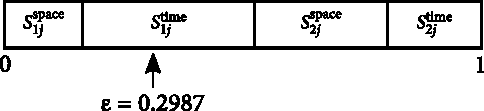
\includegraphics{figures/hidden_variables/random_choice.pdf}
    \caption{Probabilistically choosing a transition. Top: Probability flows between states in a time interval according to the three matrices of unconditional probabilities $P^\up{stay}$, $P^\up{space}$, and $P^\up{time}$ in such a way that one total unit of probability is routed from states at the initial time to states at the final time consistent with the populations resulting from quantum mechanical evolution in that timestep. Centre: The hidden variable transitions according to the corresponding conditional probabilities which are elements of the matrices $S^\up{stay}$, $S^\up{space}$, and $S^\up{time}$. Here the hidden variable is in state $1$ and we are choosing whether it will remain in that state or if it will transition to state $2$ or $3$, and if the latter, whether it transitions via a spatial or temporal non-adiabatic transition. Bottom: All the probabilities for what may happen to the hidden variable in a timestep sum to one, so an array of the cumulative probabilities can be constructed, and a random number drawn from the range $[0,1]$. The index of the smallest element of the array of cumulative sums that the random number is smaller than corresponds to the event to occur. In the above diagrammatic example, the result of the random draw is that the hidden variable is to transition to state $2$ via a spatial non-adiabatic transition.}\label{fig:random_choice}
\end{figure}

\subsubsection{Framing fewest-switches as a hidden-variable theory}

Tully's fewest-switches algorithm allows one to compute transition probabilities for a hidden variable given the Hamiltonian, the state amplitudes, and a small interval of time. Does this satisfy Aaronson's definition of a hidden variable theory? Not quite, since it requires the Hamiltonian rather than the unitary that describes state vector evolution over a particular time interval, however it is simple to reconcile the two sets of requirements. Given that the interval of time is small, the unitary describing evolution in the local basis can be linked to the effective Hamiltonian in~\eqref{eq:Tully_adiabatic_eff} via
\begin{align}
\hat U(t+\dd t, t) = \ee^{-\frac\ii\hbar\hat H_\up{eff}(\vec r, t)\,\dd t},
\end{align}
where
\begin{align}
\hat H_\up{eff} = \hat V(\vec r, t)
  - \ii\hbar\hat U(\vec r, t)\dv{t}U^\dagger_H(\vec r, t)
\end{align}
is the effective Hamiltonian in the eigenbasis of $\hat H$, the matrix representation of which can be extracted from the matrix representation of $\hat U(t+\dd t, t)$ as:
\begin{align}
H_\up{eff}(\vec r, t)\,\dd t &= \ii\hbar\Log U(t+\dd t, t)\\
&\approx \ii\hbar\left(\mathbb{I} -  U(t+\dd t, t)\right)
\end{align}
where $\Log$ is the principal value of the complex matrix logarithm.

Since only the matrix $H_\up{eff}(\vec r, t)\,\dd t$ is required to compute transition probabilities according to~\eqref{eq:fewest_switches_Heff}, and not its component terms,\footnote{Though we do need its component terms if we wish to distinguish between spatially vs.\ temporally induced transitions as in [SECREF].} specifying the initial state vector and unitary for an interval of time evolution (both in the local basis) is a sufficient input to be able to compute transition probabilities using Tully's fewest-switches algorithm. Writing the resulting matrix of probabilities in terms of $U$ gives:
\begin{align}
P_{ij} = \begin{cases}
\max\left\{0, 2\re\left(c_i^*(t)U_{ij}(t + \dd t, t)c_j(t)\right)\right\} & i \neq j\\
\abs{c_i(t)}^2 - \sum_{j\neq i} P_{ij} & i = j
\end{cases}
\end{align}
The corresponding stochastic matrix $S$ can then be obtained by scaling the columns of $P$ by the state populations as in~\eqref{eq:P_matrix_def}. Tully's fewest-switches algorithm thus satisfies Aaronson's definition of a hidden-variable theory provided that the time interval is small. What is somewhat remarkable is the low computational complexity of computing probabilities via fewest-switches. There is no matrix scaling, no matrix permanents, or any other large computational expense. It is not clear how many of Aaronson's axioms are satisfied by fewest-switches, but since it does depend on the actual coupling strengths between states via the non-adiabatic Hamiltonian, one would expect it to satisfy a few of them. Furthermore, the form of fewest-switches when framed in terms of the unitary for the given time interval is remarkably similar to that of Schr\"odinger theory. In Schr\"odinger theory one takes the absolute value of elements of $U$ and then applies row and column scalings. In fewest-switches one applies row and column scalings (explicitly given as $c_i(t)^*$ and $c_j(t)$, plus an additional factor of $2$), then takes the real part of the result and clips it to zero from below.

\subsection{Distinguishing between spatial and temporal transitions in arbitrary hidden-variable theories}

[TODO flag this as speculative and untested unless I test it]

In the above section [OR SECREF IF I MOVE THIS], we saw how to extract separate stochastic matrices from Tully's fewest-switches algorithm in order to distinguish between non-adiabatic transitions due to motion through space with a spatially varying Hamiltonian as compared to those due to the Hamiltonian's explicit time dependence. This fell naturally out of the derivation simply by not discarding the possible time-dependence of the Hamiltonian and otherwise proceeding similarly to Tully. For an arbitrary hidden variable theory however it is not so simple. In the case of Schr\"odinger theory for example, we have something of a black box which we feed unitaries and state vectors, and it gives us back stochastic matrices. It is not obvious how one might dig into the details of the matrix scaling to extract two separate conditional probabilities instead of one.

One method might be to compute a unitary as usual for the total evolution of the state vector (excluding decoherence) during a timestep, and compute $S^\up{total}$ from that according to one's hidden variable theory. Then, repeat this step, but with a unitary computed by holding the Hamiltonian's explicit time dependence constant over the timestep (allowing $\vec r$ to still vary as normal), to obtain the conditional transition probabilities $S^\up{space}$ for non-adiabatic transitions due to spatial variations alone.


[I think this won't work due to the possibility of negative probabilities. 
Probably abandon this and just use Tully's instead. Leave in the paragraph about it not being trivial though! It certainly isn't. Maybe mention that this approach doesn't always work - or maybe you could clip the probabilities to zero. But that would be privileging one type of transition over another.]

\subsection{Velocity correction and classically disallowed transitions}

When a transition of the hidden variable occurs due to a spatial non-adiabatic transition, the kinetic energy of the atom must be adjusted to conserve overall energy. The force on an atom during a transition from the $j^\up{th}$ state to the $i^\up{th}$ state due to the spatial non-adiabatic coupling term in the effective Hamiltonian is in the direction of the non-adiabatic coupling vector
\begin{align}
\vec d_{ij} &= \matrixel{\chi_i(\vec r, t)}{\nabla}{\chi_j(\vec r, t)}\\
&= \left(U_H(\vec r, t)\nabla U_H^\dagger(\vec r, t)\right)_{ij}
\end{align}
where $U_H(\vec r, t)$ is the matrix representation, in any fixed basis, of the unitary that takes state vectors into the basis in which $\hat H(\vec r, t)$ is diagonal. To conserve energy, the squared component of an atoms velocity in this direction must change by an amount:
\begin{align}
\upDelta v_{ij}^2 = \frac2m\left(V_{jj}(\vec r, t) - V_{ii}(\vec r, t)\right),
\end{align}
where $V_{ii}(\vec r, t)$ is the adiabatic potential comprising the $i^\up{th}$ spatially and/or temporally varying eigenvalue of $\hat H(\vec r, t)$. However, it is possible that a change of this size can leave an atom with a negative kinetic energy. Whilst this is quantum-mechanically permissible, it is forbidden classically, and so we simply disallow such transitions, defining a modified matrix of unconditional transition probabilities $\tilde P^\up{space}$ that sets the probability of the disallowed transitions to zero:
\begin{align}
\tilde P^\up{space}_{ij} =
\begin{cases}
P^\up{space}_{ij} & \upDelta v_{ij}^2 + \abs{\vec v\cdot\hat{\vec d_{ij}}}^2 \geq 0 \\
0 & \upDelta v_{ij}^2 + \abs{\vec v\cdot\hat{\vec d}_{ij}}^2 < 0
\end{cases}
\end{align}
where $\hat{\vec d}_{ij}$ is the unit vector in the direction of $\vec d_{ij}$.
The diagonal matrix for the probabilities of remaining in each state must be adjusted similarly to absorb the probability discarded this way:
\begin{align}
\tilde P^\up{stay}_{ii} = 
\abs{c_i(t)}^2 - \sum_{j\neq i}\left(\tilde P^\up{space}_{ij} + P^\up{time}_{ij}\right)
\end{align}
The corresponding matrices of conditional probabilities for the hidden variable transitioning, given that it is already in the $j^\up{th}$ state, are
\begin{align}
\tilde S^\up{space}_{ij} &= \frac1{\abs{c_j(t)}^2} \tilde P^\up{space}_{ij},\\
\tilde S^\up{stay}_{ij} &= \frac1{\abs{c_j(t)}^2} \tilde P^\up{stay}_{ij},
\end{align}
Of course, when making probabilistic transitions of the hidden variable, only one
column of any of the above matrices is used at a time, so the full matrices $\tilde P^\up{space}$, $\tilde P^\up{time}$, $\tilde S^\up{space}$, and $\tilde S^\up{time}$ do not need to be computed at each timestep.

In the case that a transition of the hidden variable does occur to the $i^\up{th}$ from the $j^\up{th}$ state due to a spatial non-adiabatic coupling, the velocity kick to be applied to the classical velocity vector in order to conserve momentum is:
\begin{align}
\upDelta \vec v_{ij} = \left[\sgn(\vec v\cdot \hat{\vec d}_{ij})
\sqrt{(\vec v\cdot \hat{\vec d}_{ij})^2 + \frac2m\left(V_{ii}(\vec r, t) - V_{jj}(\vec r, t)\right)} - (\vec v\cdot \hat{\vec d}_{ij}).
\right]\hat{\vec d}_{ij}
\end{align}   

\section{Decoherence}

Was not in Tully's original paper. Prior to discovering the surface hopping literature I came up with simple Markovian decoherence as a mean decoherence of thermal wavelength sized Gaussians [see section]. It is below in [SECREF]. After discovering the surface hopping literature and their fondness for spawning additional trajectories to work out decoherence more accurately, I came up with what I believe is an improvement [see subsection].

In Subsection~\ref{sec:backaction} I show the general mechanism by which the divergence of trajectories decoheres internal states of an atom, and specifically how this appears as an apparent decrease in the amplitudes of each other state when one imposes the adiabatic trajectory corresponding to one specific internal state.

\subsection{Back action of position measurement on internal state}\label{sec:backaction}

Consider an atom in a state $\ket{\Psi(t)}$, which is an arbitrary superposition of internal basis states $\ket{\chi_i}$ and motional basis states $\ket{\vec r}$: 
\begin{align}
\ket{\Psi(t)} = \int \sum_i \psi_i(\vec r, t) \ket{\chi_i}\otimes\ket{\vec r} \dd\vec r,
\end{align}
where normalisation requires that
\begin{align}
\int \sum_i \abs{\psi_i(\vec r, t)}^2 \dd\vec r = 1.
\end{align}
Recognising that $\psi_i(\vec r, t)$ is the $i^\up{th}$ component of a multi-component wavefunction that has one component for each internal state, we define (up to an arbitrary phase factor) a normalised wavefunction $\phi_i(\vec r, t)$ and corresponding motional state vector $\ket{\phi_i(t)}$ and its coefficient $c_i(t)$ for each component:
\begin{align}\label{eq:product_state_vector}
c_i(t)\phi_i(\vec r, t) &\equiv \psi_i(\vec r, t) \\
\ket{\phi_i(t)} &\equiv \int \phi_i(\vec r, t)\ket{\vec r}\dd \vec r
\end{align}
such that $\int\abs{\phi_i(\vec r, t)}^2\dd \vec r = 1$, allowing us to write our arbitrary state vector as a sum over the internal basis only:
\begin{align}
\ket{\Psi(t)} = \sum_i c_i(t) \ket{\chi_i}\otimes\ket{\phi_i(t)},
\end{align}
where the spatial state vectors $\{\ket{\phi_i(t)}\}$ are not necessarily orthogonal. To see that spatial separation of the different components leads to decoherence of the internal states, consider the pure density operator corresponding to $\ket{\Psi(t)}$:
\begin{align}
\hat\rho(t) = \ketbra{\Psi(t)}{\Psi(t)} = \sum_{ij}
c_i(t) c_j^*(t)\ketbra{\chi_i(t)}{\chi_j(t)}\otimes\ketbra{\phi_i(t)}{\phi_j(t)},
\end{align}
which we can write in the $\{\ket{\chi_i}\otimes\ket{\vec r}\} \equiv \{\ket{\chi_i\ \vec r}\} $ basis, resulting in matrix elements
\begin{align}
\rho_{ij}(t, \vec r, \vec r^\prime) &= \matrixel{\chi_i\ \vec r}{\rho(t)}{\chi_j\ \vec r^\prime},\\
&= \psi_i(\vec r, t)\psi_j^*(\vec r^\prime, t),\\
&= c_i(t) c^*_j(t) \phi_i(\vec r, t) \phi_j^*(\vec r^\prime, t).
\end{align}
A partial trace [CITE THE DECOHERENCE BOOK] over the motional degree of freedom results in a reduced density operator describing the measurement statistics of the internal degree of freedom only, assuming ignorance of the position degree of freedom:
\begin{align}
\hat\rho^\up{red}(t) &= \int\matrixel{\vec r}{\hat \rho(t) \hat {\vec r}}{\vec r}\dd \vec r\\
\Rightarrow \rho^\up{red}_{ij}(t) &= \int\rho_{ij}(t, \vec r, \vec r^\prime)\delta(\vec r - \vec r^\prime)\dd \vec r\\
&= c_i(t) c_j^*(t)\int\phi_i(\vec r, t)\phi_j^*(\vec r, t)\dd \vec r\\
&= c_i(t) c_j^*(t)\braket{\phi_j(t)}{\phi_i(t)}.
\end{align}
So we see that the off diagonals of the density matrix, representing the coherences of the internal states, are reduced by a factor $\braket{\phi_j(t)}{\phi_i(t)}$, which will be unity only for pairs of motional state vectors that are identical. We therefore see that separation in space of the wavefunctions corresponding to different internal states leads to decoherence of the internal states, with decoherence factor $r_{ji} = \braket{\phi_j(t)}{\phi_i(t)}$. This same decoherence factor appears when---instead of integrating over all positions---we project the total state vector onto a single motional state corresponding to a classical trajectory, which (along with assumptions about the form and evolution of the motional states), is how we impose classicality on the motional degree of freedom in our model. The effect of decoherence when ``following" a specific motional state through space in this way is to reduce the amplitudes of all other states not being followed by the decoherence factor between that state and the one being followed, as shown schematically in Figure [FIGREF SCHEMATIC FROM EARLIER SECTION].

Returning to our arbitrary state vector~\eqref{eq:product_state_vector}, we find (ignoring normalisation) the projected state vector $\ket{\tilde \Psi(t)} = \hat R(t)\ket{\tilde \Psi(t)}$, where $\hat R(t) = \hat 1 \otimes \ketbra{\phi_\eta(t)}{\phi_\eta(t)}$, resulting from projection of the total state vector $\ket{\Psi(t)}$ onto the specific motional state vector $\ket{\phi_\eta(t)}$ corresponding to the state selected by the hidden variable $\eta$. This gives the (non-normalised) state vector one would observe conditional on the particle being in that specific motional state at that specific time.
\begin{align}
\ket{\tilde \Psi(t)} &= \hat R(t) \ket{\Psi(t)}\\
&= \sum_i\braket{\phi_\eta(t)}{\phi_i(t)}c_i(t)\ket{\chi_i}\otimes\ket{\phi_\eta(t)}\\
&= \sum_i\tilde c_i(t)\ket{\chi_i}\otimes\ket{\phi_\eta(t)}\\
&= \ket{\tilde \chi(t)}\otimes\ket{\phi_\eta(t)},
\end{align}
where we have defined $\tilde c_i(t) = \braket{\phi_\eta(t)}{\phi_i(t)}c_i(t)$ and $\ket{\tilde \chi(t)} = \sum_i \tilde c_i(t)\ket{\chi_i}$. We can immediately see that the effect of this projection is to reduce the amplitude of all other states ($i\neq\eta$) by the decoherence factor $r_{\eta i}(t)$. We now proceed by considering this a projective measurement to have occurred at time $t$, and evolving the resulting projected state vector to time $t+\dd t$ before projecting it again:
\begin{align}\label{eq:second_proj}
\ket{\tilde \Psi(t + \dd t)} &= 
\hat R(t + \dd t)
\sum_i
\left[\tilde c_i(t) - \frac\ii\hbar\sum_j H_{ij}(t)\tilde c_j(t)\dd t\right]
\ket{\chi_i}\otimes\ket{\phi_i(t + \dd t)},
\end{align}
where $H^\up{red}_{ij}(t) = \matrixel{\chi_i}{\hat H^\up{red}(t)}{\chi_j} = \matrixel{\chi_i\ \phi_\eta(t)}{\hat H(t)}{\chi_j\ \phi_\eta(t)}$ are the elements of the ``reduced" Hamiltonian $\hat H^\up{red}(t) $ dictating the dynamics of the internal state, given the imposed motional state $\ket{\phi_\eta}$ and the total Hamiltonian $\hat H(t)$ of the system. Note that because of the previous projection already performed, all motional states $\ket{\phi_i(t)}$ were ``reset" to be equal to $\ket{\phi_\eta(t)}$ at time $t$, and therefore the evolved motional state $\ket{\phi_i(t + \dd t)}$ (the form of which we have not yet specified) represents the evolution of the motional state corresponding to the $i^\up{th}$ internal state over an interval $\dd t$, starting with the initial condition $\ket{\phi_\eta(t)}$. Accordingly, both motional states will still be approximately equal after this short evolution, allowing us to write
\begin{align}
\braket{\phi_\eta(t + \dd t)}{\phi_i(t + \dd t)} &= \braket{\phi_\eta(t)}{\phi_i(t)} + \dv{t}\braket{\phi_\eta(t)}{\phi_i(t)}\dd t\\
& = 1 + \dv{r_{\eta i}(t)}{t}.
\end{align}
Using this fact in applying the projection in~\eqref{eq:second_proj} yields a product state once more:
\begin{align}\label{eq:second_proj}
\ket{\tilde \Psi(t + \dd t)} &= 
\sum_i
\left(1 + \dv{r_{\eta i}(t)}{t}\right)
\left[\tilde c_i(t) - \frac{\ii}\hbar\sum_j H_{ij}(t) \tilde c_j(t)\dd t\right]
\ket{\chi_i}\otimes\ket{\phi_\eta(t + \dd t)}\\
\Rightarrow \ket{\tilde \chi(t + \dd t)} &= \sum_i
\left(1 + \dv{r_{\eta i}(t)}{t}\right)
\left[\tilde c_i(t) - \frac{\ii}\hbar\sum_j H_{ij}(t) \tilde c_j(t)\dd t\right]
\ket{\chi_i}
\end{align}
which we can solve for $\frac1{\dd t}\left(\ket{\tilde \chi(t + \dd t)} - \ket{\tilde \chi(t)}\right)$ to obtain a differential equation for $\ket{\tilde \chi(t)}$:
\begin{align}
\dv{t} \ket{\tilde \chi(t)} =
\left[-\frac\ii\hbar\hat H^\up{red}(t) - \hat\Gamma(t)\right]\ket{\tilde\chi(t)},
\end{align}
where $\hat\Gamma(t)$ is a diagonal operator in the $\{\ket{\chi_i}\}$ basis with diagonals
\begin{align}
\Gamma_{i}(t) = -\dv{r_{\eta i}(t)}{t} = -\dv{t} \braket{\phi_\eta(t)}{\phi_i(t)},
\end{align}
which are \emph{decoherence rates}, and cause exponential damping of all internal states other than the $\ket{\chi_\eta}$ state, with faster damping the faster the motional state corresponding to a given internal state diverges with $\ket{\phi_\eta(t)}$.

\subsection{Reframing as continuous weak measurement of internal state}

[Write the set of operators and their probabilities. Talk about the speculative stuff here]

This projection onto a single (albeit still quantum) motional state is the first step toward imposing classicality on the motional degree of freedom of our system, and is is similar, but not identical to performing a continuous weak quantum measurement of the position degree of freedom. Similarly to the case of continuous weak measurement, we have a set of (time dependent in our case) projection operators $\{\Omega_i(t)\}$ with
\begin{align}
\Omega_i(t) = \hat 1 \otimes \int\psi_i(\vec r, t)\ketbra{\vec r}{\vec r} \dd \vec r,
\end{align}
and are choosing from them at each timestep with probability of the $i^\up{th}$ outcome being $\matrixel{\Psi(t)}{\Omega_i^\dagger(t)}{\Omega_i(t)}$. This is as if we were performing a measurement with hypothetical measurement device not capable of distinguishing different positions perfectly, but only of determining which of the (not necessarily orthogonal) motional state vectors $\{\ket{\phi_i(t)}\}$ the system is in. 

Essentially at each timestep we are performing a weak measurement (a positive operator valued measure or POVM [CITE]) of the position degree of freedom, with a hypothetical measurement device that cannot distinguish positions perfectly, and has measurement outcomes corresponding to the set of motional states $\{\ket{\phi_i}\}$.

[ELABORATE. WRITE THE POVMS AND THEIR PROBABILITIES]

The measurement outcome is not selected randomly at the time the projection is performed, but instead pre-ordained by the current value of the hidden variable $\eta$. The fact that the hidden-variable makes stochastic transitions in a manner consistent with the Born rule guarantees that the probability of each measurement outcome is the same as if we had chosen an outcome randomly based on the Born rule itself at the time of each measurement. See Section [SECREF SPECULATIVE ASIDE] for a discussion of why use of a hidden variable is preferable to actually using the Born rule.

Effectively performing this measurement at each timestep of a simulation means that we are assuming that any amplitude leaving the envelope of the currently tracked motional state will either not come back into it, or will have a minimal effect if it does. Given the six-dimensional size of phase space, in which two separated pieces of amplitude of an atom's wavefunction must find each other if they are to interfere, this is a worthy approximation in many cases, to the extent that until recently [CITE]it was not possible to observe such interference in the case of Stern--Gerlach separation of cold atoms. The problem of getting the wavepackets back together again is called the ``Humpty Dumpty problem" and was a serious concern to early atom interferometry researches before the use of Bragg pulses [CITE] allowed experiments to create large momentum differences between wavepackets without having them more slowly traverse the intermediate regions of momentum space where they might accumulate coherence-destroying phase noise.

\subsection{Form of the decoherence factor and the quantum Zeno effect}

Finally we will say something about the motional states $\{\ket{\phi_i(t)}\}$. We will assume that each of them is a Gaussian wavepacket with width equal the thermal wavelength, or a specific coherence length we will define, whichever is smaller (see Section [WRITE SECTION HOW BIG IS A WAVEPACKET?]). Each wavepacket moves, without dispersion, with its mean position subject to the adiabatic potential $V_{ii}(\vec r, t)$ as described in in [SECREF TIME DEPENDENT FORMULATION OF TULLY]. Thus:
\begin{align}
\braket{\vec r}{\phi_i(t)} &= \phi_i(\vec r, t) = A\ee^{-\frac{\abs{\vec r - \vec r_i(t)}^2}{4\sigma^2} + \ii \frac m\hbar \vec v_i(t)\cdot (\vec r - \vec r_i(t))}\\
\dv{t} \vec r_i(t) &= \vec v_i(t)\\
\dv{t} \vec v_i(t) &= -\frac1m\nabla V_{ii}(\vec r_i, t).
\end{align}
Where $A$ is a real normalisation constant.\footnote{The overall phase is determined by the offset $\vec r - \vec r_i(t)$ in the second term in the exponent, and is chosen such that $\phi_i(\vec r, t)$ is real at $\vec r=\vec r_i$, which ensures that $\braket{\phi_i(t)}{\phi_j(t)}$ has a phase depending only on the relative positions of the two wavepackets rather than their distance from some arbitrary origin. Acquiring an additional arbitrary phase at each timestep when we apply our reduction operator $\hat R$ would not affect the system dynamics, but is unappealing nonetheless.} This gives for our decoherence factor:
\begin{align}
R_{ij}(t) = \ee^{-\left(\frac1{8\sigma^2}\abs{\vec r_{ij}}^2
+ \frac\ii 2 \vec r_{ij}(t) \cdot \vec k_{ij}(t) + \frac{\sigma^2}{2} \abs{\vec k_{ij}(t)}^2
\right)},
\end{align}
where $\vec r_{ij}(t) = \vec r_i(t) - \vec r_j(t)$ and $\vec k_{ij}(t) = \frac m\hbar \left(\vec v_i(t) - \vec v_j(t)\right)$ are the relative mean position and wavevector of the pair of wavepackets. As expected, it is equal to unity when the two wavepackets have identical positions and velocities, and decays to zero for increasing relative position and velocity. 

[TODO: Flag in intro that I will summarise the necessary equations later in the algorithm section, and make sure you do that]

But now we arrive at a problem. Because all the motional states are reset to be equal to $\ket{\phi_\eta(t)}$ at each timestep, the relative position and wavevector of the two wavepackets are both zero at all times, and so our decoherence rates are [TODO: rename ``naive" decoherence rate?]:
\begin{align}
\Gamma_{ij}(t) &= -\left[\dv{R_{ij}(t)}{t}\right]_{
\stackon[1pt]
{$\scriptscriptstyle\, \vec v_{ij} = 0$}
{$\scriptscriptstyle\, \vec k_{ij} = 0$}
}\\
&= -\left[
\pdv{R_{ij}(t)}{\vec r_{ij}}\cdot \dv{\vec r_{ij}(t)}{t} + 
\pdv{R_{ij}(t)}{\vec k_{ij}}\cdot \dv{\vec k_{ij}(t)}{t}\right]_{
\stackon[1pt]
{$\scriptscriptstyle\, \vec v_{ij} = 0$}
{$\scriptscriptstyle\, \vec k_{ij} = 0$}
}\\
&= -\left[
2\vec k_{ij}R_{ij}(t)\cdot\dv{\vec k_{ij}(t)}{t}\right]_{
\stackon[1pt]
{$\scriptscriptstyle\, \vec v_{ij} = 0$}
{$\scriptscriptstyle\, \vec k_{ij} = 0$}
}\\
&= 0.
\end{align}
Every decoherence rate is zero. What is going on? The answer is the quantum Zeno effect [CITE LOADS OF THINGS], which is the name given to the fact that, in the limit of infinitely frequent measurements of whether quantum evolution has occurred, the back action of the measurement has the effect of preventing the evolution from occurring at all. One saying is that ``A watched quantum pot never boils" [CITE?]. In our case, the fact that we are projecting constantly onto our assumed set of motional states causes the amplitude flows to the other motional states to be exactly zero. The appearance of the quantum Zeno effect ought to be a reminder that the assumption of infinitely frequent projective measurements is unphysical. In our case it certainly is---we have merely imagined a hypothetical measurement device collapsing our position states because we don't want to simulate them, not because any such measurement device actually exists. Nonetheless the internal states of the atom \emph{do} decohere even in the absence of measurement (and there is eventual measurement when the atoms collide with other atoms or otherwise interact with anything in a position-dependent way), and we wish to model the approximate effect of this.

Note that if the decoherence factor had the form of exponential decay:
\begin{align}
R^\up{Markovian}_{ij}(t) = e^{-\gamma_{ij} t}, 
\end{align}
then the decoherence rate would be the constant $\gamma_{ij}$, and not zero. This is the case for Markovian decoherence, which is when the environment has no memory of its past interaction with the system. The memory in our case is that the wavepackets accelerate away from each other, starting from zero relative position and velocity at each timestep---the relative position and velocity comprise a memory of the past interaction, which we are erasing each time we reproject.

The lack of an environmental memory is only ever approximately true, and no decoherence factors in nature have the form of a decaying exponential at all times. At small enough times the overlap between two states can only move away from unity quadratically owing to unitary evolution on account of the Schr\"odinger equation, guaranteeing an initial time derivative of zero for all physical decoherence factors. However in many systems of interest, the specifics of the interaction with the system are quickly forgotten by the environmental states, and the decoherence factor does approach a decaying exponential. This is the case, for example, for spontaneous photon emission by atoms, which one can consider a measurement effect in which the electromagnetic field is being regularly measured by the environment in the photon number basis. In the various quantum trajectories methods used to simulate atoms in the presence of spontaneous emission, if one assumes that the measurements are projective, one must simply assume that the frequent measurements take place at large enough timescales that the decoherence factor is in the exponential decay regime, provided that this is much smaller than other dynamical timescales, which is true for spontaneous emission. This can be recast as a continuous \emph{weak} measurement, rather than infrequent projective measurements [CITE THE STRAIGHTFORWARD INTRODUCTION], which is more physically realistic than the assumption of projective measurements at somewhat arbitrarily chosen intervals, but results in the same differential equations.

A decoherence factor that has the form of a decaying exponential implies that any chosen measurement interval results in the same fractional reduction in state amplitudes, since the differential equation $\dv{\tilde c_{i}(t)}{t} = -\gamma \tilde c_i(t)$ has the solution $\tilde c(t) = e^{-\gamma t} \tilde c(0)$, that is, repeated consideration of only the first part of the decoherence factor ends up tracing out the whole decoherence curve over time.

How can we replicate something like this for our separating wavepackets? I have two approaches. 

[move this to the other section on non-Markovian decoherence?]

Firstly we need to generalise our conception of the decoherence rate. We have assumed so far that the motional states are being ``reset" after each projective measurement to be equal to $\ket{\phi_\eta(t)}$ at each timestep. What is the reduction in the state amplitudes at each timestep if the wavepackets do not reset, but are left as arbitrary states for the time being? We know that if we were to perform a projective measurement at time $t$, the $i^\up{th}$ state amplitude would be reduced by a factor of $R_{\eta i}(t)$ compared to the original state amplitude $c_i(t)$:
\begin{align}
\tilde c_i(t) = R_{\eta i}(t) c_i(t).
\end{align}
This implies:
\begin{align}
\dv{\tilde c_i(t)}{t} &= \dv{R_{\eta i}(t)}{t} c_i(t)\\
&= \frac1{R_{\eta i}(t)}\dv{R_{\eta i}(t)}{t} \tilde c_i(t).
\end{align}
and so we see that a a decoherence rate that does not reset the environment states is the (negative of the) logarithmic derivative of the decoherence factor, rather than just its derivative. This case encompasses the earlier case in which $R_{\eta i}(t) = 1$ at all times, in which case the logarithmic and ordinary derivatives are the same.

\subsection{Approximate Markovian decoherence}

A crude way to include decoherence is just to [assuming wavepackets are separating with constant acceleration, move this stuff here?] approximate $R_{\eta i}(t)$ as a decaying exponential with approximately the right decay constant. This is crude because $R_{\eta i}(t)$ does not look much like a decaying exponential [see figure FIGREF]. In the limit of large $t$, its functional form is $e^{-t^4}$, not the exponential decay required to treat the decoherence as Markovian at any timescale.

To find an approximate Markovian decoherence rate, we first construct a ``time ignorant" decoherence factor $\tilde R_{\eta i}(t)$ that answers the question ``What is the expected value of $R_{\eta i}(t)$ at all times $t > 0$ if I don't know how long before $t=0$ the two wavepackets began separating?" We can then take the derivative of this time-ignorant decoherence factor at $t=0$ to use as an approximate Markovian decoherence rate $\Gamma^\up{Markovian}_i$. Whilst extremely approximate, this method of including decoherence is nonetheless an improvement over the Ehrenfest method (which has no decoherence), and over Tully's original fewest-hops surface hopping method [CITE], which also lacked any decoherence. Others [CITE HEAPS, LOOK AT REVIEW ARTICLE FOR A LIST MAYBE] have since introduced approximate damping of states in a manner very similar to that presented in this subsection, but I was unaware of these developments when I developed this method.

Proceeding, we define the time-ignorant decoherence factor $\tilde R_{ij}(t)$ as the average\footnote{Not a quantum expectation value, just a weighted sum.} of all decoherence factors one would obtain if the two wavepackets began separating at some point in time before $t=0$:
\begin{align}
\tilde R_{ij}(t) &= A\int_{-\infty}^0\braket{\phi_i(t-t^\prime)}{\phi_j(t - t^\prime)} \,\dd t^\prime\\
&= A\int_{-\infty}^0 R(t-t^\prime) \,\dd t^\prime
\end{align}
where $A$ is a normalisation constant such that $\tilde R_{ij}(0) = 0$, and where we take that $\ket{\phi_i(0)} = \ket{\phi_j(0)}$ with each thereafter evolving according to the classical motion of their centre of mass as in [EQUATIONS].

[Notation is a bit shoddy - specify that motional states are dependent on a trajectory? How can I fit that in the notation?]

[Mention earlier that the form of $R(t)$ depends on the separation time and is classical evolution of v and t. This will fit right in with the definitions of dv/dt etc.]

[Make gamma have ij subscripts again with the DE - maybe - think about this]

Our time-ignorant decoherence rate is then the (negative of the) derivative of $\tilde R_{ij}(t)$ at $t=0$:
\begin{align}
\Gamma_i^\up{Markovian} = -\frac{\left[\dv{t}\int_{-\infty}^0 R(t-t^\prime) \,\dd t^\prime\right]_{t=0} }
{\left[\int_{-\infty}^0 R(t-t^\prime) \,\dd t^\prime\right]_{t=0}}.
\end{align}
Moving the derivative inside the integral, noting that $\dv{R(t - t^\prime)}{t} = \dv{R(t - t^\prime)}{t - t^\prime}$ and setting $t = 0$, we get:
\begin{align}
\Gamma_i^\up{Markovian} &= -\frac
{\int_{-\infty}^0 R^\prime(-t^\prime) \,\dd t^\prime}
{\int_{-\infty}^0 R(-t^\prime) \,\dd t^\prime}\\
&= -\frac
{\int_0^\infty R^\prime(t^\prime) \,\dd t^\prime}
{\int_0^\infty R(t^\prime) \,\dd t^\prime}
\end{align}
where $R^\prime$ is the derivative of $R$ with respect to its argument. By the fundamental theorem of calculus the numerator is $-1$, since $R(t)$ decreases from unity at $t=0$ to zero as $t$ goes to infinity, leaving us with:

\begin{align}
\left(\Gamma_i^\up{Markovian}\right)^{-1} &= 
  \int_0^\infty R(t^\prime) \,\dd t^\prime\\
&= \int_0^\infty \ee^{-\left(\frac1{8\sigma^2}\abs{\vec r_{ij}}^2
+ \frac\ii 2 \vec r_{ij}(t^\prime) \cdot \vec k_{ij}(t^\prime) + \frac{\sigma^2}{2} \abs{\vec k_{ij}(t^\prime)}^2
\right)} \,\dd t^\prime
\end{align}

[FIX $\vec r_{ij}$ - ``rel"? Gah.]

Approximating the motion of the wavepackets as moving away from each other with constant acceleration based on the adiabatic potentials at position $\vec r$ and time $t$ gives:
\begin{align}
\vec r_{ij}(t^\prime) = \frac12\vec a_{ij}(\vec r, t) {t^\prime}^2
\end{align}
and
\begin{align}
\vec k_{ij}(t^\prime) = \frac m \hbar \vec a_{ij}(\vec r, t) t^\prime,
\end{align}
where the relative acceleration is
\begin{align}
\vec a_{ij}(\vec r, t) = -\frac1 m\left(\nabla V_{ii}(\vec r, t) - \nabla V_{jj}(\vec r, t)\right).
\end{align}
\subsection{Continuously spawned mean auxiliary trajectories}

My fancy cool model which is awesome and rad.

\begin{align}
\vec r_{i\neq\eta}(t + \dd t) &= \frac{\sum_j \tilde P_{ij}\vec r_j(t)}
{\abs{c_i(t+\dd t)}^2},\\
\vec v_{i\neq\eta}(t + \dd t) &= \frac{\sum_j 
\left((P^\up{time}_{ij} + \tilde P^\up{stay}_{ij})\vec v_j(t)
+ \tilde P^\up{space}_{ij}(\vec v_i + \upDelta \vec v_{ij})\right)}
{\abs{c_i(t+\dd t)}^2}.
\end{align}


\section{Algorithm}

\subsection{Further approximations}

say that H is based on centre of mass of the eta component


Specifics of the algorithm, now that everything is defined.
\begin{itemize}
    \item Schr\"odinger HVSC: with either Markovian decoherence, or auxilliary trajectories. No time dependence allowed

    \item Fewest hops HVSC/surface hopping: either with Markovian decoherence or
    auxilliary trajectories. Time dependence allowed!

\end{itemize}
\section{results}
Pretty results go here

\section{Discussion and conclusion}

Although the method wasn't original, in rediscovering it I have identified that hidden variable theories and hopping algorithms are in fact the same thing. I am relieved that I can use a hidden variable theory that is numerically faster to compute then Schrodinger theory and wonder what the implications are for Aaronson's ideas, given the reasoning outlined in the intro that hidden variable theories ought to be hard to compute. In addition, my decoherence method totally kicks butt and the time dependence thing is nifty.

Discuss how it would make sense for the systems to behave in the presence of collisions w.r.t collapse of state vectors.

\subsection{Speculative aside: Monte-Carlo wavefunctions and Stochastic Schr\"odinger equations} 
The Stochastic Schr\"odinger equation [CITE] is very similar to the case where the measurement outcome is chosen at projection time, randomly each time rather than according to a hidden variable. This produces the same eventual transition probabilities, but is not suitable for us. If we moved the atom according to the force experienced by the state

\section{Approximate Markovian decoherence rate for separating wavepackets}

Positional separation of two different internal states of an atom leads to decoherence of those states, with a decoherence factor $R_{ij}(t)$ equal to the overlap of the spatial wavefunctions of the two components in question a time $t$ after they began separating. Approximating both wavepackets as initially overlapping Gaussians of width $\sigma$, ignoring dispersion, and assuming they separate with constant relative acceleration $a_{ij}$, the decoherence factor is

\begin{align}
R_{ij}(t) &= \braket{\psi_i(t)}{\psi_j(t)}\\
 &= C \int_{-\infty}^{\infty} e^{-\frac{x^2}{4\sigma^2}}e^{-\frac{(x-x_\up{rel})^2}{4\sigma^2} + ik_\up{rel}x}\,\dd x,\label{eq:gaussian_integral}
\end{align}
where
\begin{align}
x_{\mathrm{rel}}(t) = \frac12a_{ij}t^2
\end{align}
and
\begin{align}
k_\up{rel}(t) = \frac m \hbar a_{ij} t
\end{align}
are the wavepackets' relative\footnote{$a_{ij}$, $x_\up{rel}$ and $k_\up{rel}$ are the acceleration, position, and wavenumber of the $j^\up{th}$ component with respect to the $i^\up{th}$ component, that is, $a_{ij} = a_j - a_i$, etc.} position and wavenumber due to acceleration for a time $t$ starting from zero relative velocity, and
\begin{align}
C^{-1}=\int_{-\infty}^\infty e^{-\frac{x^2}{2\sigma^2}}\,\dd x\label{supp:eq:Cdef}
\end{align}
is a normalisation constant [TODO CHECK IF NEEDS TO BE SQUARED]. Note that this expression holds for any number of dimensions---relative motion is only along one axis so the integrals in all other directions equal one.

Evaluating the Gaussian integral \eqref{eq:gaussian_integral} gives the following expression for the decoherence factor $R_{ij}(t)$:
\begin{align}
R_{ij}(t)&= e^{-\left[
        \frac{1} {8\sigma^2} x_\up{rel}^2
      + \frac i2 x_{\mathrm{rel}} k_\up{rel}
      + \frac{\sigma^2}{2} k_\up{rel}^2
      \right]}\label{eq:decoherence_factor}.
\end{align}

This is a decoherence \emph{factor}; it is the factor by which the $(i, j)$ off-diagonal of the reduced density matrix for the atom's internal state will be reduced at time $t$. The corresponding decoherence \emph{rate} is given by the logarithmic derivative of \eqref{eq:decoherence_factor}:

\begin{align}
\Gamma_{ij}(t) = - \frac 1 {R_{ij}(t)} \dv t {R_{ij}(t)}.
\end{align}

 The fact that \eqref{eq:decoherence_factor} does not describe a constant decoherence rate (i.e., it does not have the functional form of exponential decay) means that the back action on the atom's internal state caused by measurements of its motional state will be different depending on the interval of time between measurements.

For example, the logarithmic derivative of \eqref{eq:decoherence_factor} approaches zero as $t$ goes to zero. This means that in the limit of infinitely frequent measurements, no decoherence occurs at all in between measurements, and the motional state is reset after each measurement such that the wavepackets never separate at all. This is the quantum Zeno effect, and its appearance in models of open quantum systems is usually treated as a reminder that the assumption of infinitely frequent strong measurements is unphysical [CITE].

Since experimentally we are not measuring atoms' motional states so frequently, we ought to wait until the wavepackets are completely separated before performing a projective measurement. As in quantum optics models of open quantum systems, in which the measurement interval ``should be large enough to allow the photons to get away from the atom" [CITE The Quantum Jump Approach
and Quantum Trajectories Gerhard C. Hegerfeldt], ours should be large enough for the atomic states to get away from each other.

If at large enough times, a decoherence rate is independent of time, that decoherence is called Markovian at that timescale. A Markovian environment is one that has no memory of the decoherence process---it ``forgets" any information caused by past interaction with the system. Even though at short times, all decoherence rates in quantum mechanics tend to zero [CITE], if they become Markovian on a timescale shorter than other timescales of interest, the Markov approximation can be used and a constant decoherence rate used at all times. In quantum optics, the decoherence factor for the internal state of an atom due to photon emission indeed tends to exponential decay on timescales that are still much shorter than that of the system evolution, and thus the Markov approximation is accurate.

Unlike quantum optics models, our decoherence factor does not describe Markovian decoherence on any timescale. In the limit of large $t$, its functional form is $e^{-t^4}$, not the exponential decay required to treat the decoherence as Markovian [CITE] at that timescale. Nonetheless, if we wish to write a time-local differential equation for the internal state of the atom, Markovian decoherence is the only kind we can include [CITE].

To that end, we will now construct a ``time ignorant" version of $R_{ij}(t)$ that answers the question ``What is the expected decoherence factor at all future times, if you don't know how long it has been since the two wavepackets began separating?" In this way we can compute an \emph{average} decoherence rate $\Gamma_{ij}$ described by our decoherence factor, even though $R_{ij}(t)$ does not have a constant decoherence rate at large times. This essentially amounts to finding the best fitting exponential to $R_{ij}(t)$. Whilst this approximation is crude, it is nonetheless an improvement over the Ehrenfest model, which has no decoherence at all (i.e. it has a decoherence rate that is also constant like ours---but equal to zero).

\begin{figure}[t]
    \centerfloat
    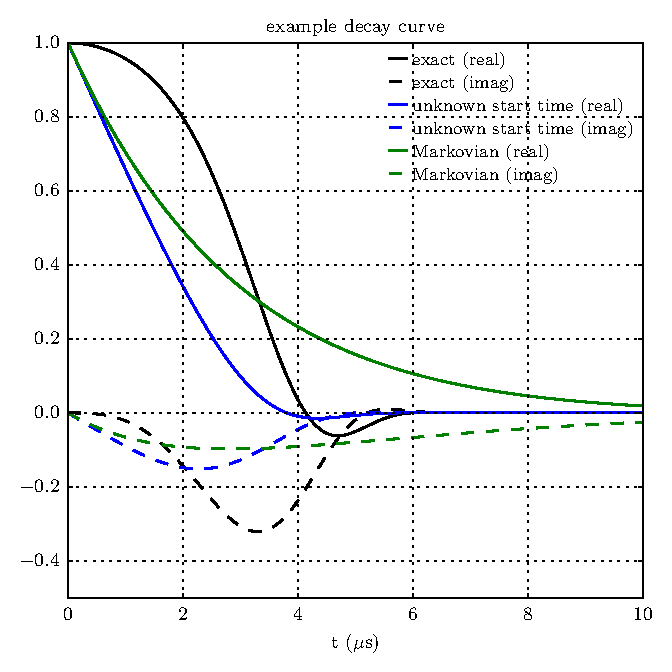
\includegraphics{figures/hidden_variables/decoherence_factor_example.pdf}
    \caption{Caption.}
    \label{fig:decoherence_factor_example}
\end{figure}

We define the time-ignorant decoherence factor $\tilde R_{ij}(t)$ as the overlap of the wavefunction of the $i^\up{th}$ internal state with a superposition of wavepackets of the $j^\up{th}$ internal state, with the superposition being over all times in the past the wavepackets began separating:
\begin{align}
\tilde R_{ij}(t) &= \bra{\psi_i(t)} A\int_{-\infty}^0 \ket{\psi_j(t - t^\prime)} \,\dd t^\prime\\
\end{align}
where $A$ is a normalisation constant such that $\tilde R_{ij}(0) = 1$.
Since $\ket{\psi_i(t)}$ is time independent (rather, since we can perform our calculations in the frame of reference in which it is stationary), this is:
\begin{align}
\tilde R_{ij}(t) &= A\int_{-\infty}^0 R_{ij}(t - t^\prime) \,\dd t^\prime,
\end{align}
which is simply the convolution of our decoherence factor with a step function which is nonzero at all negative times.
Our average decoherence rate $\Gamma_{ij}$ is then given by the logarithmic derivative of $\tilde R_{ij}(t)$ at $t=0$:

\begin{align}
\Gamma_{ij} &= -\frac {\tilde R_{ij}^\prime(0)} {\tilde R_{ij}(0)}\\
&= -\frac {\int_0^\infty \tilde R_{ij}^\prime(t)\,\dd t} {\int_0^\infty \tilde R_{ij}(t)\, \dd t}\\
\Rightarrow \Gamma_{ij}^{-1}&= \int_0^\infty e^{-\left[
        \frac{1} {8\sigma^2} x_\up{rel}^2
      + \frac i2 x_{\mathrm{rel}} k_\up{rel}
      + \frac{\sigma^2}{2} k_\up{rel}^2
      \right]}\, \dd t.\label{eq:gamma_integral}
\end{align}

As mentioned, $\Gamma_{ij}$ is the decay constant for the best fitting exponential to our decoherence factor \eqref{eq:decoherence_factor}. Although \eqref{eq:decoherence_factor} looks nothing like a decaying exponential in time, an exponential approximation to it nonetheless ought to decay to zero on the same timescale. An example of this is shown in \figref{fig:decoherence_factor_example}

In order to obtain an approximate analytic expression for this integral, we consider two limiting cases and then stitch them together in the intermediate regime. In the limit of small wavepackets, $\sigma$ is small and thus the first term in the exponent in \eqref{eq:gamma_integral} is largest, and the third term is smallest. In this regime, which describes when positional separation (as opposed to separation in $k$-space) dominates the decoherence, we'll neglect the third term in the exponent and treat the second term as small relative to the first.
This gives us:
\begin{align}
\Gamma_{ij\,\up{(pos)}}^{-1} &\approx \int_0^\infty e^{-\left[
        \frac{1} {8\sigma^2} x_\up{rel}^2
      + \frac i2 x_{\mathrm{rel}} k_\up{rel}
      \right]}\, \dd t.\\
      &\approx \int_0^\infty e^{-
              \frac{1} {8\sigma^2} x_\up{rel}^2}\left(1 - \frac i2 x_{\mathrm{rel}} k_\up{rel}\right)\, \dd t.\label{eq:gamma_pos_exp}\\
      &= 2^{\frac54}\upGamma(\tfrac54)\sqrt{\frac{\sigma}{a_{ij}}} - 2i\frac{m \sigma^2}{\hbar},\label{eq:gamma_pos_recip}
\end{align}
where we used a first-order Taylor expansion of an exponential in \eqref{eq:gamma_pos_exp}. We similarly use a first order expansion to take the reciprocal of \eqref{eq:gamma_pos_recip} (since the second term is much smaller than the first\footnote{This isn't necessary in order to obtain a simple expression for $\Gamma_{ij\,\up{(pos)}}$---the reciprocal without this approximation is equally simple---but it leaves us with power laws for the real and imaginary parts of $\Gamma_{ij\,\up{(pos)}}$, which are easier to stitch together with those from the large $\sigma$ regime.}), and arrive at:
\begin{align}
\Gamma_{ij\,\up{(pos)}} &\approx \frac1{2^{\frac54}\upGamma(\tfrac54)}\sqrt{\frac{a_{ij}}{\sigma}}
+ \frac i {2\sqrt{2}\upGamma(\tfrac54)^2} \frac{m\sigma a_{ij}}{\hbar}\label{eq:gamma_pos_final}%\\
% &\approx 0.463865\sqrt{\frac{a_{ij}}{\sigma}}
% + 0.430341 i \frac{m\sigma a_{ij}}{\hbar}.
\end{align}

Similarly for the large $\sigma$ regime, we neglect the first term in the exponent of \eqref{eq:gamma_integral} and consider the second term small relative to the third. This is the regime in which the decrease in overlap of the two wavepackets is dominated by their separation in velocity space. Following the same process as above gives:
\begin{align}
\Gamma_{ij\,\up{(vel)}}^{-1} &\approx \int_0^\infty e^{-\left[
        \frac i2 x_{\mathrm{rel}} k_\up{rel}
        + \frac{\sigma^2}{2} k_\up{rel}^2
      \right]}\, \dd t.\\
      &\approx \int_0^\infty \left(1 - \frac i2 x_{\mathrm{rel}} k_\up{rel}\right)
      e^{-\frac{\sigma^2}{2} k_\up{rel}^2}\, \dd t\\
      & = \sqrt{\frac\pi2}\frac\hbar{m \sigma a_{ij}} - i\frac{\hbar^3}{2m^3 \sigma^4 a_{ij}^2}\\
      \Rightarrow \Gamma_{ij\,\up{(vel)}} &\approx \sqrt{\frac2\pi}\frac{m \sigma a_{ij}}\hbar
                                          + \frac i\pi \frac\hbar{m \sigma^2}
                                          \label{eq:gamma_vel_final}
\end{align}
Equations \eqref{eq:gamma_pos_final} and \eqref{eq:gamma_vel_final} are our final expressions for the docoherence rate in the limit of small and large wavepackets respectively. Adding their real parts in quadrature and adding the reciprocals of their imaginary parts then provides a reasonable approximation for $\Gamma_{ij}$ over all wavepacket sizes:
\begin{align}
\Gamma_{ij} \approx
\left[\re(\Gamma_{ij\,\up{(pos)}})^2 + \re(\Gamma_{ij\,\up{(vel)}})^2\right]^{\frac12}
+ i\left[\im(\Gamma_{ij\,\up{(pos)}})^{-1} + \im(\Gamma_{ij\,\up{(vel)}})^{-1}\right]^{-1}.
\label{eq:gamma_total}
\end{align}

\begin{figure}[t]
    \centerfloat
    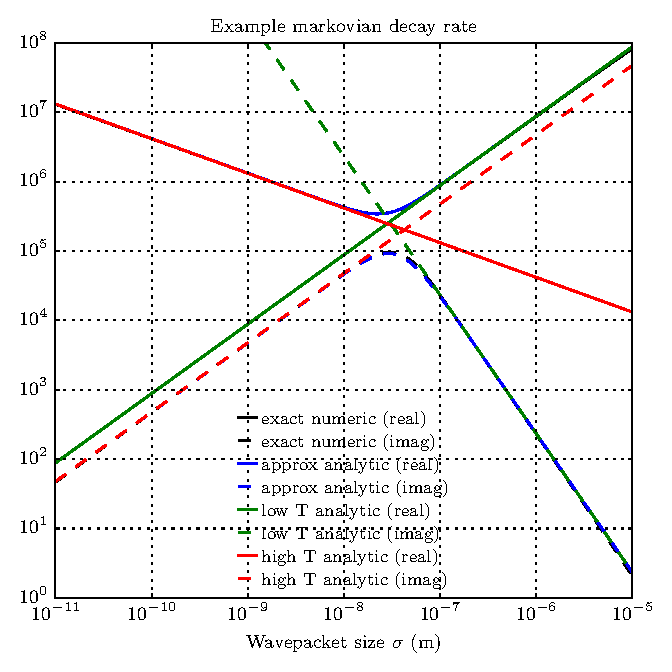
\includegraphics{figures/hidden_variables/decoherence_rate_example.pdf}
    \caption{Caption.}\label{fig:decoherence_rate_example}
\end{figure}

We now have an approximate analytic expression that is computationally inexpensive to evaluate for each atom in an ensemble at every timestep of a differential equation.
An example showing the accuracy of \eqref{eq:gamma_total}, compared to the exact expression \eqref{eq:gamma_integral} for $\Gamma_{ij}$ over a range of wavepacket sizes is shown in \figref{fig:decoherence_rate_example}.

\section{Choice of wavepacket size}

How big is a wavepacket? Be sure to say it's the thermal wavelength except not too big because the single mode approximation won't be valid otherwise. 
